\begin{abstract}
People read books every day, both to enjoy themselves and to learn. Many people and organizations own quite the amount of books, and want to share these. It is difficult for these people and organizations to share books, without any way of tracking the loans or which books are available. This was presented as the topic for a project for a group in the course TDT4290 at NTNU, who was given the task of developing a system that met this need. 

This report presents how the project was organized, the tools the group used, how the product was built using the Lean Startup as a basis, what the final product looked like, how it worked and how it met the demands and needs of the customer.

The report is based upon the work of that group, who during 12 weeks developed an Android and iOS application, as well as a \gls{backend} solution that can help users all over the world share their books, and their knowledge. Books are added and shared by either scanning the barcode, or searching with text. The users can also find books to borrow by looking through their joint groups. The solution is called CrowdShelf.
\\
\\
\\
{
\begin{center}
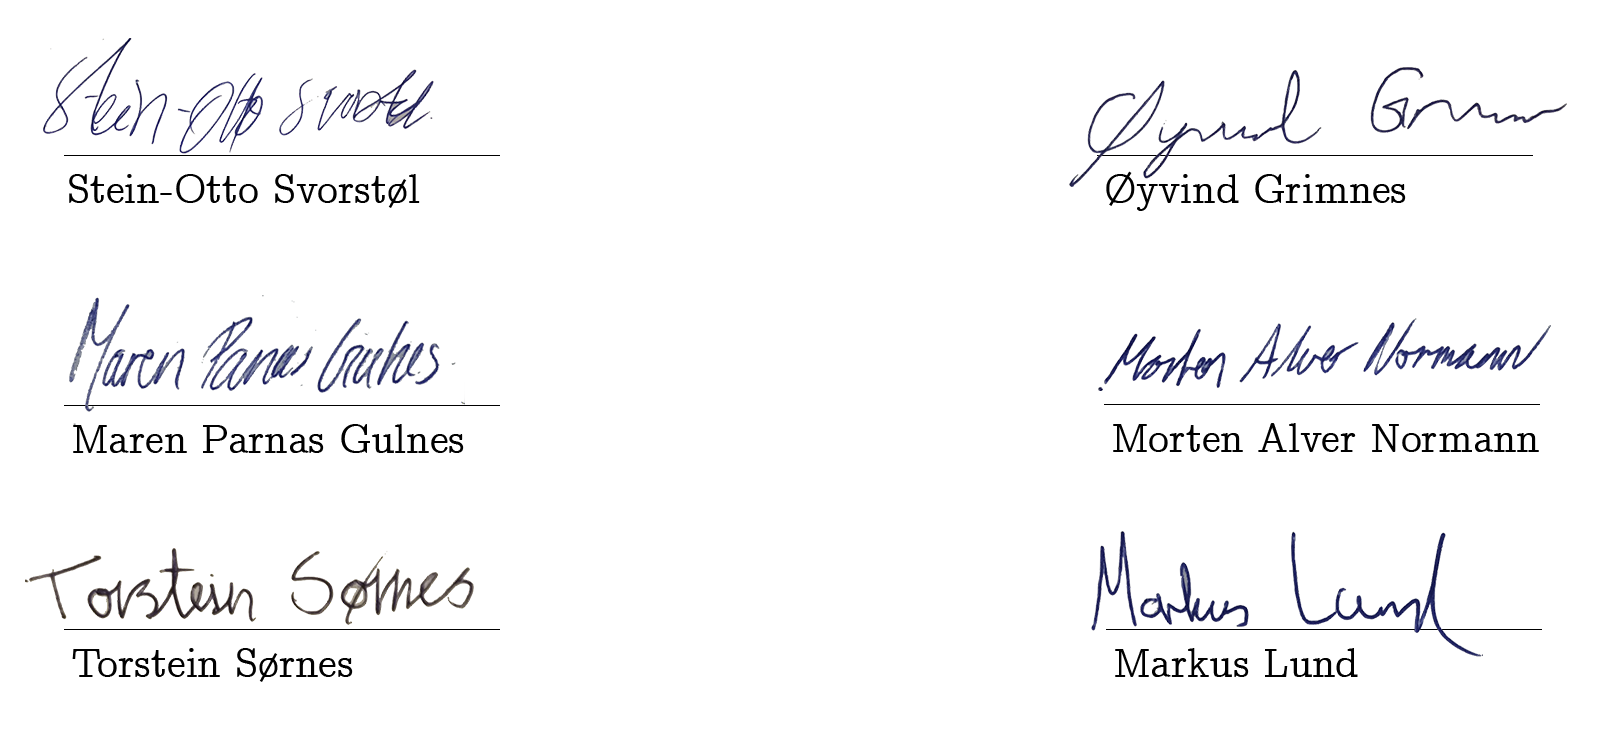
\includegraphics{figs/Signatures.png}
\par
\end{center}
}

\end{abstract}

% ref https://en.wikipedia.org/wiki/Abstract_(summary)#Abstract_Types